\chapter{Optimization and Resampling Algorithms} \label{chp:optimization}
%\epigraph{Great quote.}{Author}
\begin{figure}[H]
	\centering
	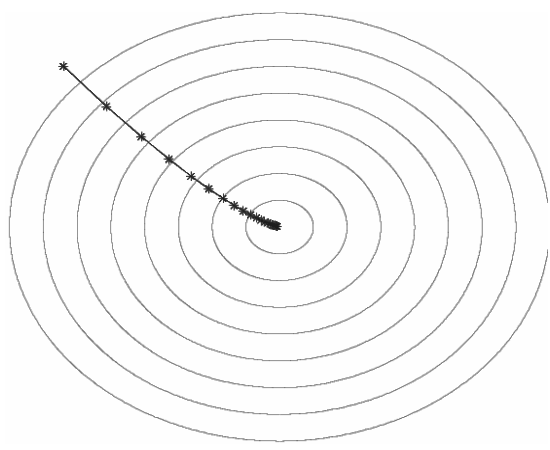
\includegraphics[scale=0.4]{Images/gd_bw.png}
	\caption{An iterative optimization algorithm is always approaching an extremum in a possibly multi-dimensional space. Here illustrated in a two-dimensional space where the equipotential curves are drawn.}
\end{figure}

In this chapter, we will cover the remaining algorithms we need before we can move on to the implementation. First of all, a good optimization algorithm is a must in order to obtain the correct minimum of the cost function. For our purpose, we potentially have thousands of parameters to optimize, and therefore a robust optimizer is required. The ADAM optimizer has proven its ability to solve similar problems, and we will therefore have a thoroughly discussion of the algorithm.

Secondly, we need an algorithm to determine the statistical errors with high precision. This is the task of the resampling methods, where we keep our attention on the blocking method. For long, the blocking method suffered from the need of tailored hyper-parameters, but the recent years automated blocking methods have been developed, in particular by Marius Jonsson \cite{jonsson_standard_2018}. We will explain the idea behind the traditional blocking method, and in the code we use the automated blocking algorithm. 



\section{Summary of the algorithms} \label{sec:algorithmsummary}
Up to this point we have presented several algorithms that contribute to the variational Monte-Carlo algorithm, and to give the reader a complete description of the simulating procedure, we will here summarize them and place them in the correct order. First, Metropolis-Hastings algorithm was given, which is responsible for the sampling. Thereafter, we presented a few optimization algorithms, before the blocking algorithm was given. 

The optimization loop forms the outer environment of the algorithm, which means that for every time we update the parameters, we run a set of Monte-Carlo cycles. The expectation values found throughout those cycles are used to update the parameters. Further, the blocking algorithm is used to approximate the uncertainties of the expectation values. In algorithm \ref{alg:total}, a simple variational Monte-Carlo algorithm is presented in its entirety. For simplicity, we present the Brute-Force Metropolis algorithm and standard gradient descent. 

\IncMargin{1em}
\begin{algorithm}
	\SetAlgoLined
	
	\Parameter{$\eta$: Learning rate}
	\Parameter{$\Delta x$: Step length}
	\Require{$\Psi_T(\bs{r},\bs{\theta})$: Trial wave function}
	\BlankLine
	$\bs{r}\leftarrow \mathcal{N}(0,\sigma^2)$ (Initialize positions randomly)\;
	$\bs{\theta}\leftarrow \mathcal{U}(0,1)$ (Initialize parameters, could be randomly)\;
	\While{not converged}{ 
		$\bs{E}\leftarrow[-]$ (Declare an empty local energy list)\;
		$\bs{d}_{\theta}\leftarrow[-]$ (Declare an empty parameter gradient list)\;
		$\bs{Ed}_{\theta}\leftarrow[-]$ (Declare an empty list containing parameter gradient $\cdot$ local energy)\;
		\For{$i\leftarrow 1$ \KwTo $M$}{
			$\bs{r}\leftarrow\bs{r}+\Delta x$ (Update position)\;
			\If{$\Psi_T(\bs{r}_{\text{new}})/\Psi_T(\bs{r}_{\text{old}})<\mathcal{U}(0,1)$}{
				reject move \;
			}
			$E^i\leftarrow \big(\hat{\mathcal{H}}\Psi_T(\bs{r},\bs{\theta})\big)/\Psi_T(\bs{r},\bs{\theta})$ (Fill $\bs{E}$-list with local energies) \;
			$d_{\theta}^i\leftarrow \nabla_{\theta}\ln\Psi_T(\bs{r})$ (Fill $\bs{d}_{\theta}$-list with parameter gradients) \;
			$Ed_{\theta}^i\leftarrow \bs{E}^i\cdot\bs{d}_{\theta}^i$ (Fill $\bs{Ed}_{\theta}$-list) \;
		}
		$\bs{E}_0\leftarrow \bs{E}$\;
		$i\leftarrow 0$ (Initial blocking step)\;
		\While{$\text{var}(\bs{E}_{i+1})\neq \text{var}(\bs{E}_{i})$}{
			$n_i\leftarrow n/2^i$ (Number of elements in $\bs{E}_i$)\;
			$\text{var}(\bs{E}_i)\leftarrow\sigma_i^2/n_i$ (Estimate the variance of $\bs{E}_i$)\;
			\For{$k\leftarrow 1$ \KwTo $n_i$}{
				$(\bs{E}_{i+1})_k\leftarrow0.5\big((\bs{E}_i)_{2k-1}+(\bs{E}_i)_{2k}\big)$ (The blocking transformations)\;
			}
			$i\leftarrow i+1$ (Increase $i$ for each iteration)\;
		}
		$\overline{\bs{E}}\leftarrow\sum_{j=1}^ME^j/M$ (Compute the local energy sample mean)\;
		$\overline{\bs{d}}_{\theta}\leftarrow\sum_{j=1}^Md_{\theta}^j/M$ (Compute the sample mean of $\bs{d}_{\theta}$)\;
		$\overline{\bs{Ed}}_{\theta}\leftarrow\sum_{j=1}^MEd_{\theta}^j/M$ (Compute the sample mean of $\bs{Ed}_{\theta}$)\;
		$G_{\theta}\leftarrow2\big(\overline{\bs{Ed}}_{\theta}-\overline{\bs{E}}\cdot\overline{\bs{d}}_{\theta}\big)$\;
		$\bs{\theta}\leftarrow \bs{\theta}-\eta\cdot G_{\theta}$\;
	}
	\KwResult{An estimate of the many-body wave function $\Psi(\bs{r})$ and the local energy $\langle E_L\rangle\approx\overline{\bs{E}}$ with its uncertainty $\text{var}(\overline{\bs{E}})$.}
	\caption{The variational Monte-Carlo algorithm in its simplest form. The outer loop is for the parameter update. The first inner loop is the sampling where $M$ is the number of Monte-Carlo cycles, and the last inner loop is the resampling loop. Note that we present the brute-force Metropolis algorithm, while the more robust Metropolis-Hasting algorithm, found in algorithm \ref{alg:hastings}, is preferred. Furthermore, we also limit us to the simple gradient descent method. $\mathcal{N}(\mu,\sigma)$ denotes a normal distribution with mean $\mu$ and variance $\sigma$, while $\mathcal{U}(0,1)$ denotes a uniform distribution between 0 and 1. }
	\label{alg:total}
\end{algorithm} \DecMargin{1em}







